\chapter{Related Work}\label{related-work}
The work presented in this thesis is based on two main areas of research: evaluation of LLMs(LLMs) and Information Retrieval(IR).
In this chapter, the current state of research in those areas is presented, as it relates to this thesis.
We start with a short introduction to LLMs, then present the current evaluation methods for those models in the field of question answering, since the different versions of question answering tasks, especially long form question answering are most similar to our evaluation setup.
\\
Afterwards, the field of IR is introduced.
Different retrieval methods used in this thesis are presented and why they were chosen for this work.
Additionally, the evaluation metrics used to compare those retrieval methods are introduced.

\section{Evaluation of LLMs for Question Answering}\label{sec:evaluation-of-large-language-models}
Transformer-based language models are generally defined as systems that produce probability distributions over a set of tokens(which can be words, subwords or characters) given the preceding or surrounding context.    
The rise of LLMs started with the introduction of the transformer architecture by \cite{vaswani:2017}, followed by the release of models like BERT~(\cite{devlin:2018}) and GPT-2~(\cite{radford:2018}).
The transformer architecture allowed the models to process more context than previous models, such as LSTM-based methods like ELMo~(\cite{peters:2018}), or static word embeddings based on statistical co-occurrences like GloVe~(\cite{pennington:2014}).
This led to improvements in many NLP tasks over earlier methods, as shown by \cite{radford:2018}, who compare the base GPT performance against multiple then state-of-the-art models on different tasks, improving or performing at least competitively on all of them.
\\
With the release of GPT-3~(\cite{brown:2020}), the size of datasets used to train LLMs, as well as the number of parameters in the models, increased to a point where the models are able to produce coherent text on a wide range of tasks.

This meant, that models had to be evaluated on all of those tasks, leading to the development of new evaluation benchmarks.
In this section, we want to focus on the current evaluation methods of Question Answering capabilities of LLMs.
\\
The task of Question Answering (QA) is not clearly defined in the context of LLMs.
In the beginning, for models like BERT and the first version of GPT, the task was to answer questions based on a given context, by selecting a span of text from the context.
The next versions of models focused on answering multiple choice questions, where the model had to select the correct answer from a set of possible answers.
This could be done either with context, or without.
Additionally, models were evaluated on questions where the answers are single numbers, entities or other versions of "fill in the blank" questions.
\\
Those versions of QA all have in common, that they are relatively easy to evaluate.
Overlap with the answer span can be calculated, or the correct answer can be compared to the predicted answer.
However, with the capabilities of LLMs expanding version by version, the task of free form question answering gained more importance.
Here, models are evaluated on their ability to answer questions in a free form manner, without any constraints on the answer.
Answers can get long and complex, branching out in different directions by including examples or other information.
The evaluation of such answers is not as straightforward as for the other versions of QA, so human evaluation is the gold standard.
\\
In the following, the different QA versions will be introduced, including popular datasets and evaluation metrics for them.

\subsection{Extractive Question Answering}\label{sec:extractive-qa}
\begin{figure}[h]
    \centering
    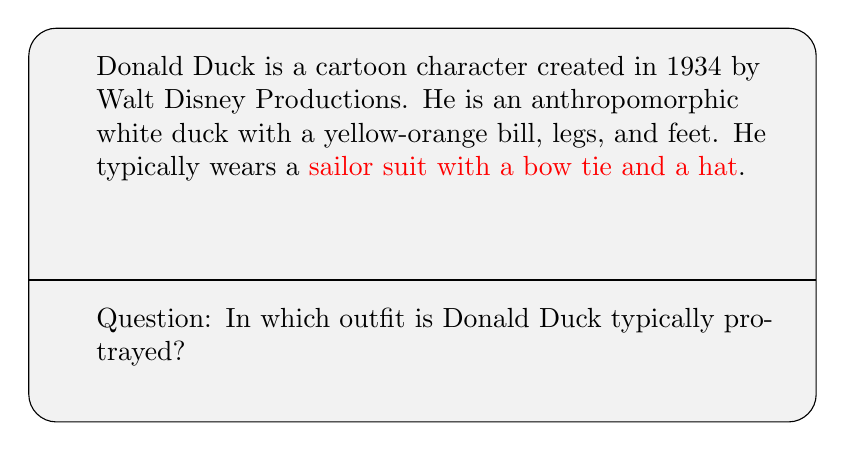
\begin{tikzpicture}
        % Draw paper background
        \draw[fill=gray!10,rounded corners=1em] (0,0) rectangle (10,5);
        % Draw text
        \node[align=left,anchor=north west, text width=9cm,inner sep=1em] at (0.5,5.0) {
            Donald Duck is a cartoon character created in 1934 by Walt Disney Productions. He is an anthropomorphic white duck with a yellow-orange bill, legs, and feet. He typically wears a \textcolor{red}{sailor suit with a bow tie and a hat}.
        };
        % Draw vertical line
        \draw[thick] (0,1.8) -- (10,1.8);
        % Draw question
        \node[align=left,anchor=north west, text width=9cm,inner sep=1em] at (0.5,1.8) {
            Question: In which outfit is Donald Duck typically protrayed?
        };
    \end{tikzpicture}
    \caption{Example of a typical extractive question answering task: The answer span "sailor suit with a bow tie and a hat" is highlighted in red in the paragraph.}
    \label{fig:extractive_qa_example}
\end{figure}
Extractive QA is the task of answering questions, given a context containing the answer.
In this context, which can be a short paragraph or entire Wikipedia article, the correct answer span has to be selected by the model.
Some benchmarks include unanswerable questions, where the model has to predict, that the question cannot be answered from the given context.
\\
One of the most popular datasets for evaluating LLMs in this task is SQuAD~(\cite{rajpurkar:2016}), and its successor SQuAD 2.0~(\cite{rajpurkar:2018}), which includes unanswerable questions.
Many other datasets like NarrativeQA~(\cite{kovcisky:2018}), QuAC~(\cite{choi:2018}) or Natural Questions~(\cite{kwiatkowski:2019}) are based on the same principle.
They consist of questions written by crowd workers or experts in the field, based on a Wikipedia article snippet or similar text passages.
The exact constraints on the questions and the context vary between the datasets, but the general idea is the same.
A typical example is shown in Figure~\ref{fig:extractive_qa_example}.
\\
The evaluation metrics for tasks of this category are based on the overlap between the predicted answer span and the ground truth answer span.
Specifically, this would be the exact match (EM) score, which measures the percentage of exact matches between the predicted and the ground truth answer span, or the F1 score, which measures the average overlap between the tokens in the two spans.
\\
For earlier LLMs like BERT, this meant that for each word in the context, the model had to predict the probability of it being the start or end of the answer token.~(\cite{devlin:2018})
To achieve this, the model was fine-tuned on the SQuAD dataset. 
\\
Later models like GPT-3 were able directly generate the answer from the context and the questions without any fine-tuning, by using the zero-shot, single-shot or multi-shot capabilities of the model.~(\cite{brown:2020})
In some settings of the datasets, the context can be completely omitted, forcing the model to directly answer the question.
This means that the results of the two approaches are not directly comparable, because even tough the models were evaluated on the same dataset, the approaches are fundamentally different.

\subsection{Multiple Choice Question Answering}\label{sec:multiple-choice-qa}
\begin{figure}[h]
    \centering
    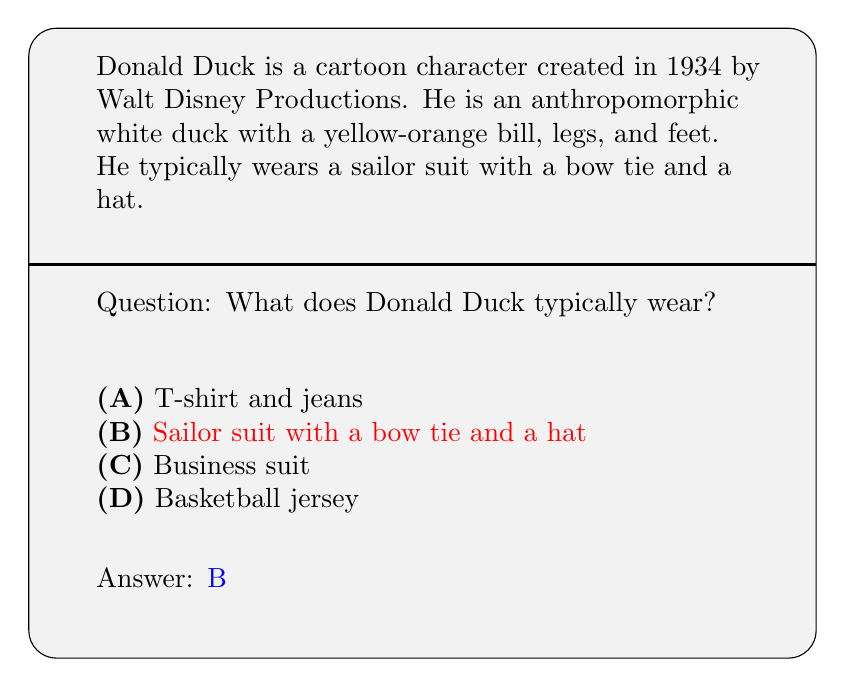
\begin{tikzpicture}
        % Draw paper background
        \draw[fill=gray!10,rounded corners=1em] (0,0) rectangle (10,8);
        % Draw text
        \node[align=left,anchor=north west, text width=8.5cm,inner sep=1em] at (0.5,8.0) {
            Donald Duck is a cartoon character created in 1934 by Walt Disney Productions. He is an anthropomorphic white duck with a yellow-orange bill, legs, and feet. He typically wears a sailor suit with a bow tie and a hat.
        };
        % Draw vertical line
        \draw[thick] (0,5) -- (10,5);
        % Draw question
        \node[align=left,anchor=north west, text width=8.5cm,inner sep=1em] at (0.5,5) {
            Question: What does Donald Duck typically wear?
        };
        % Draw multiple-choice options
        \node[align=left,anchor=north west, text width=8.5cm,inner sep=1em] at (0.5,3.8) {
            \textbf{(A)} T-shirt and jeans \\
            \textbf{(B)} \textcolor{red}{Sailor suit with a bow tie and a hat} \\
            \textbf{(C)} Business suit \\
            \textbf{(D)} Basketball jersey
        };
        \node[align=left,anchor=north west, text width=9cm,inner sep=1em] at (0.5,1.5) {
            Answer: \textcolor{blue}{B}
        };
    \end{tikzpicture}
    \caption{Example of a Multiple Choice with context: The correct multiple-choice option is highlighted in red.
    The blue B would be a possible answer generated by the LLM, after being primed with the context and the question.
    }
    \label{fig:mc_example}
\end{figure}
For multiple choice question answering, the model has to select the correct answer from a set of possible answers, which can be done with or without context.
A multple choice sample including context is shown in Figure~\ref{fig:mc_example}.
Some datasets include questions with multiple possible answers, so that the model has to check each answer for correctness, not only find the best fitting answer.
Questions for these tasks often stem from official exams, like the MMLU dataset~(\cite{hendrycks:2020}), which combines question from many exams like the United States Medical Licensing Examination or the Examination for Professional Practice in Psychology.
In other datasets, the questions are collected from crowd workers and verified by experts~(\cite{clark:2018},~\cite{mihaylov:2018}).
\\
Evaluation in this task is straightforward, since the model has to select the correct answer from a set of possible answers, making accuracy the most common metric.
For evaluating LLMs, that means selecting the answer option for which the model assigns the highest probability, after being primed with few-shot examples and prompted by \emph{'Answer: '} after the last question and answer options.

\subsection{Long Form Question Answering}\label{sec:long-form-qa}
\begin{figure}[h]
    \centering
    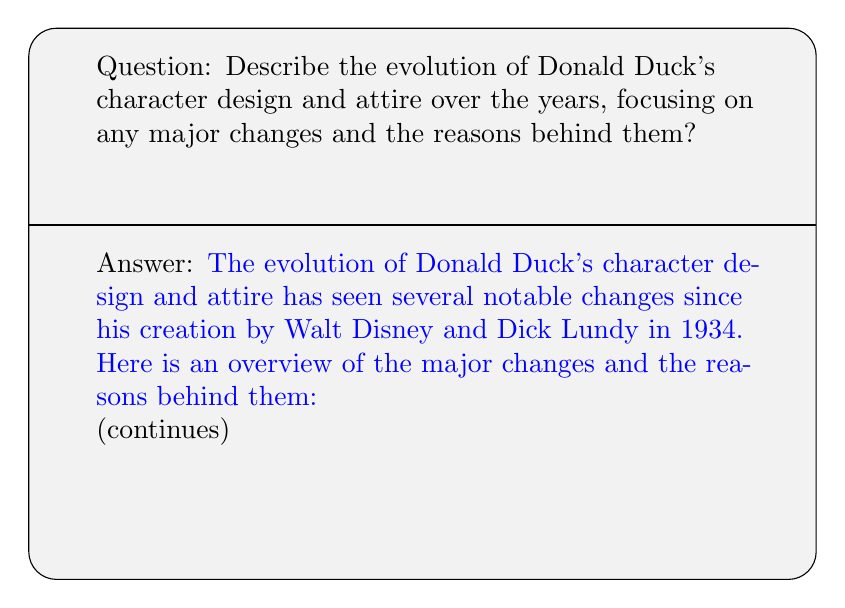
\begin{tikzpicture}
        % Draw paper background for question
        \draw[fill=gray!10,rounded corners=1em] (0,0) rectangle (10,7);
        % Draw question
        \node[align=left,anchor=north west, text width=8.5cm,inner sep=1em] at (0.5,7) {
            Question: Describe the evolution of Donald Duck's character design and attire over the years, focusing on any major changes and the reasons behind them?
        };
        % Draw vertical line
        \draw[thick] (0,4.5) -- (10,4.5);
        % Draw sample answer
        \node[align=left,anchor=north west, text width=8.5cm,inner sep=1em] at (0.5,4.5) {
            Answer: \textcolor{blue}{The evolution of Donald Duck's character design and attire has seen several notable changes since his creation by Walt Disney and Dick Lundy in 1934. Here is an overview of the major changes and the reasons behind them:}
            \\
            (continues)
        };
    \end{tikzpicture}
    \caption{Example of Long-Form QA without Context: The question prompts for a detailed answer about Donald Duck's character evolution and attire. The prompt given to the model is written in black, the sample answer (generated by ChatGPT-3.5) is written in blue.}
    \label{fig:long_form_qa_example_with_answer}
\end{figure}

This task of freely answering complex questions, which can't be answered by one entity or number, but require a longer, more nuanced answer.
Originally, this task stems from the IR community, where the model has to retrieve a document or a set of documents, which contain the answer to the question.

In some cases, those documents are then summarized to produce the final answer.
With LLMs being deployed in chatbots and as such expected to deliver answers mostly without context, the task of long form question answering was adapted to this setting.
\\
So far, only a handful of datasets are available for this task, with the first dataset in this category being the ELI5 dataset~(\cite{fan:2019}).
It consists of questions and the corresponding highest voted answer from the "Explain Like I'm Five" subreddit, where users ask questions about complex topics, which are then answered by other users.
They are accompanied by support documents, which are retrieved from web sources by querying for the original question.
This dataset was used to by~\cite{nakano:2021} to fine-tune GPT-3 for the task of long form question answering, without using the context documents.
The answers given by the fine-tuned model are evaluated by humans, by comparing them to the highest voted answer from the ELI5 dataset.
\\ 
An additional dataset for this task is the MultiMedQA~(\cite{singhal:2023}), which curates questions from multiple other datasets used previously. 
Answers generated by physicians are used as ground truth answers.
Those are then compared to the model generated answers by other physicians, as well as by laypeople.
Additionally, the answers were individually rated in different rubrics, introduced in a previous work~(\cite{singhal:2022}).
\\
None of the release papers for current, main-stream LLMs like GPT-3~(\cite{brown:2020}), GPT-4~(\cite{openai:2023}) or Llama 2~(\cite{touvron:2023}) include evaluations on common benchmarks for this category.
This shows, that long form question answering is still a relatively new task, lacking academic benchmarks.

\subsubsection{Difficulties of Long Form Question Answering}\label{sec:long-form-qa-difficulties}

Recent works have shown multiple challenges in the task of long form question answering, independently of which model architecture is used to answer the questions.
Since the answers are free form text, and not just a multiple choice option, one number or one entity, the quality of the model can't be measured using accuracy or similar metrics.
Multiple evaluation dimensions are of interest, adding for example relevance and understandability to the correctness dimension of other question answering tasks.
\\\\  

\cite{xu:2023} focus on the evaluation process of LFQA, comparing different automatic evaluation methods to human judgement.
They differentiate between general-purpose generation evaluation metrics, which were originally designed for other NLP tasks like summarization or translation, and fine-tuned metrics, which are fine-tuned to LFQA.
The following types of metrics are considered general-purpose metrics, used in the same way in different NLP tasks:
\begin{itemize}
\item \textbf{Answer-reference metrics:} Include like ROUGE or BERTScore. These metrics compare generated answers to reference answers, focusing on aspects like lexical overlap and semantic similarity.
\item \textbf{Answer-only metrics:} Such as Self-BLEU measure the fluency and diversity of generated text. These are intrinsic metrics of the generated text and do not need a reference answer for evaluation.
\item \textbf{Question-answer metrics:} Score answers given the question in one of two ways: either by calculating the likelihood of questions given an answer, or by using an encoder model to score sequences given a prefix.
\item \textbf{Answer-evidence metrics:} Judge the given answer by the evidence documents used to generate it. This method indirectly assesses the answer's credibility and factual accuracy.
\end{itemize}
In addition to those general metrics, \cite{xu:2023} evaluate two different versions of fine-tuned metrics.
The first one is based on Longformer~(\cite{beltagy:2020}), in which the model is fine-tuned to produce a score given a question and an answer, optionally combined with evidence documents.
The second model is a fine-tuned version of GPT-3, which is trained to output either \emph{Answer1} or \emph{Answer2} given a question and two answer options.
Both fine-tuned models are trained on the dataset generated by \cite{nakano:2021}, which contains human preference labels for different answer pairs.
\\
All automatic evaluation methods are evaluated on the task of choosing the preferable answer given two long form answers to a question.
The results are compared to previous human judgement on the same task.
They find that one of their baseline models, choosing always the longest answer, performs nearly as good as the fine-tuned GPT3 model, which outperformed all other methods.
Both variants are still outperformed by human agreement, which is the gold standard.
\\\\
\cite{krishna:2021} investigate in more detail the problems of reference based evaluation metrics like ROUGE-L. 
They highlight, that those metrics are unable to capture answer components like examples, if those examples are not present in the ground truth answers. 
\\
Furthermore, they note that even human evaluation is limited in judging LFQA over different models.
Some problems include the hiring process of experts, especially when datasets tackle multiple fields of expertise.
Finding experts of similar education and background is challenging, when doing evaluations of different models over a span of time.
Additionally, the evaluation process is more mentally challenging for the individual annotator the longer the answers get.
Similar problems have previously been shown by \cite{akoury:2020} in the context of machine generated stories.
They find that crowd workers have low agreement for different evaluation metrics when evaluating the same stories.
They tackle this problem by using gamification techniques to activate online users of a story writing platform to evaluate and improve the generated stories.
A similar approach is taken by \cite{dugan:2020}, who implement a website where users try to differentiate machine-generated text from human generated text.
\\\\
This shows that there are still many obstacles to overcome in the task of evaluating long form question answering systems.
Since our approach of tackling this problem uses concepts from the field of information retrieval, a short overview of relevant methods is given in the next section.
\\
TODO More precise summary and better transition to next section
%------------------------------------------------------------------
%------------------------------------------------------------------
%------------------------------------------------------------------

\section{Retrieval Models}\label{sec:retrieval-models}
Since we want to use retrieval methods to evaluate the performance of LLMs, we will give some background on  the field of IR, and how it relates to long form question answering.
Information retrieval (IR) is the process of retrieving relevant information from a collection of documents.
This can be in the form of whole documents, passages or single sentences.
Usually, the document corpus is first indexed, transforming the documents into a form that is more suitable for retrieval.
This includes tokenization, stemming, stop word removal and other preprocessing steps.
Commonly, an inverted index is then created, which maps each term in the corpus to the documents that contain it.
Now, given a query, an IR system returns a ranked list of documents that are most relevant to the query.
To achieve this, IR systems estimate a usefulness score for each document in the collection with respect to the query.
The documents are then ranked according to their usefulness scores, with the most relevant documents appearing at the top of the list.
Some pipelines include a re-ranking step, in which the most relevant documents are re-ranked after the first retrieval, as shown in Figure~\ref{fig:reranking_pipeline}.
\begin{figure}[tb]
\centering
\begin{tikzpicture}[node distance=0.8cm, auto]

% Styles for boxes
\tikzstyle{box} = [rectangle, draw, fill=blue!10, text width=4.5em, text centered, rounded corners, minimum height=3em]
\tikzstyle{user} = [ellipse, draw, fill=blue!30, text width=4.5em, text centered, rounded corners, minimum height=3em]

% Nodes
\node [box, fill=blue!30] (corpus) {Document Corpus};
\node [box, fill=blue!30, right=of corpus] (index) {Index};
\node [box, fill=blue!30, right=of index] (model) {Retrieval Model};
\node [user, above=of model] (query) {Queries};
\node [box, fill=blue!5, right=of model] (rerank) {Re-ranking};
\node [box, fill=blue!30, right=of rerank] (output) {Output};

% Edges
\draw[->] (corpus) -- (index);
\draw[->] (query) -- (model);
\draw[->] (index) -- (model);
\draw[->] (model) -- (rerank);
\draw[->] (rerank) -- (output);

\end{tikzpicture}
\caption{Depiction of a basic retrieval pipeline, with optional re-ranking step. The process begins with a document corpus, which is indexed to facilitate efficient retrieval. Given the information need of a user in the form of a query, the retrieval model returns the most relevant documents. Optionally, the documents can be re-ranked using a re-ranking model which is usually more resource intensive.}
\label{fig:reranking_pipeline}
\end{figure}

\subsection{Baseline Retrieval Models}\label{sec:baseline-retrieval-models}
First, we will look at the basic retrieval models, which are used as baselines in this thesis.
They have been chosen, because they were shown to be effective on the used dataset in previous work~(\cite{goeuriot:2021}).
Both models use the implementation in the Terrier IR platform~(\cite{ounis:2005}).

\subsubsection{TF-IDF}\label{sec:tf-idf}
Term Frequency-Inverse Document Frequency (TF-IDF) is one of the most prevalent weighting schemes in information retrieval.
It aims to measure the importance of a term in a document relative to a collection of documents or corpus.
The central intuition is that terms that appear frequently in a document but not in many other documents in the corpus are significant and thus should be given higher weight.
\\\\
Given a term \( t \) and a document \( d \) in a corpus \( D \):
\[ \text{TF-IDF}(t, d, D) = \text{TF}(t, d) \times \text{IDF}(t, D) \]
Where \( \text{TF}(t, d) \) is the term frequency of term \( t \) in document \( d \) and 
\[ \text{IDF}(t, D) = \log \left( \frac{|D|}{1 + \text{df}(t, D)} \right) \]
with \( |D| \) being the total number of documents in the corpus and \( \text{df}(t, D) \) is the number of documents containing term \( t \).
\\
In the actual retrieval step, a similarity score between the terms in the query and the documents is calculated based on all terms TF-IDF scores.
The documents are then ranked according to their similarity to the query.
\\
In the Terrier IR platform, the implementation of TF-IDF uses variants of the TF and IDF components.
For Term Frequency, the Robertson's TF formulation~(\cite{robertson:2004}) is used, which incorporates an additional parameter, that adds a saturation effect to the term frequency.
For IDF, the original formulation by Sparck Jones~(\cite{sparck:1972}) is applied.

\subsubsection{DPH}\label{sec:dph}
Divergence from Randomness (DFR) is a framework in information retrieval that assigns term weights based on the divergence of the actual within-document term frequency distribution from a random term frequency distribution~(\cite{amati:2006}).
The DPH (Divergence from randomness using the Hyper-geometric distribution model) is one of the models derived from the DFR framework.
\\
The principle behind DFR is that terms that are informative in a document will have a distribution that deviates significantly from what would be expected if terms were distributed randomly.
While TF-IDF emphasizes the importance of terms based on their frequency in a document and their inverse frequency in the corpus, DPH focuses on the divergence of a term's distribution from what would be expected under a random distribution.
Specifically, DPH assesses the divergence using the hyper-geometric distribution.
In essence, where TF-IDF weights terms based on their prominence and rarity, DPH weights them based on how much their occurrence pattern deviates from randomness.
The implementation in the Terrier IR platform follows the original formulation by \cite{amati:2006}.


\subsection{Transformer-based Retrieval Models}\label{sec:transformer-retrieval-models}
As mentioned in earlier sections, transformer-based models have been shown to be effective on a variety of tasks, including information retrieval.
There are different approaches of how transformers can be used for retrieval, a brief overview of methods used in this thesis is given here.
\\\\
Two of the most common transformer based architectures are cross-encoder and bi-encoder models.
\begin{figure}[h]
  \centering
  % Define colors
  \definecolor{textcolor}{RGB}{255, 230, 204}
  \definecolor{encodercolor}{RGB}{204, 229, 255}
  \definecolor{embeddingcolor}{RGB}{217, 234, 211}
  \definecolor{scorecolor}{RGB}{230, 204, 255} % New color for scores

  % Bi-Encoder
  \begin{minipage}{.48\textwidth}
    \centering
    \begin{tikzpicture}[node distance=0.7cm, auto, every node/.style={scale=0.8}]
      \tikzstyle{text_in} = [rectangle, rounded corners, minimum width=3cm, minimum height=1cm, align=center, draw=black, fill=textcolor]
      \tikzstyle{encoder} = [rectangle, rounded corners, minimum width=3cm, minimum height=1cm, align=center, draw=black, fill=encodercolor]
      \tikzstyle{embedding} = [rectangle, rounded corners, minimum width=3cm, minimum height=1cm, align=center, draw=black, fill=embeddingcolor]
      \tikzstyle{score} = [ellipse, minimum width=2cm, minimum height=1cm, align=center, draw=black, fill=scorecolor]

      % Nodes
      \node[text_in] (query) {Query};
      \node[encoder, below=of query] (qencoder) {Query Encoder};
      \node[embedding, below=of qencoder] (qembed) {Query Embedding};
      
      \node[text_in, right=of query, xshift=1cm] (doc) {Document};
      \node[encoder, below=of doc] (docencoder) {Doc Encoder};
      \node[embedding, below=of docencoder] (docembed) {Doc Embedding};

      \node[score, below=of qembed.south, xshift=2.5cm] (biScore) {Relevance Score}; % New node for relevance score

      % Arrows
      \draw[-{Latex[length=3mm]}] (query) -- (qencoder);
      \draw[-{Latex[length=3mm]}] (qencoder) -- (qembed);
      \draw[-{Latex[length=3mm]}] (qembed) -- (biScore);
      \draw[-{Latex[length=3mm]}] (doc) -- (docencoder);
      \draw[-{Latex[length=3mm]}] (docencoder) -- (docembed);
      \draw[-{Latex[length=3mm]}] (docembed) -- (biScore);

    \end{tikzpicture}
    \caption{Bi-Encoder Architecture. Query and document are encoded separately, then the relevance is calculated based on similarity measures between the embeddings.}
  \end{minipage}
  \hfill
  % Cross-Encoder
  \begin{minipage}{.48\textwidth}
    \centering
    \begin{tikzpicture}[node distance=0.7cm, auto, every node/.style={scale=0.8}]
      \tikzstyle{text_in} = [rectangle, rounded corners, minimum width=3cm, minimum height=1cm, align=center, draw=black, fill=textcolor]
      \tikzstyle{encoder} = [rectangle, rounded corners, minimum width=3cm, minimum height=1cm, align=center, draw=black, fill=encodercolor]
      \tikzstyle{embedding} = [rectangle, rounded corners, minimum width=3cm, minimum height=1cm, align=center, draw=black, fill=embeddingcolor]
      \tikzstyle{score} = [ellipse, minimum width=2cm, minimum height=1cm, align=center, draw=black, fill=scorecolor]

      % Nodes
      \node[text_in, right=] (query) {Query};

      \node[text_in, right=of query, xshift=1cm] (doc) {Document};

      \node[text_in, below=of query.south, xshift=2.5cm] (qdoc) {Query $+$ Document};

      \node[encoder, below=of qdoc] (qencoder) {Cross-Encoder};

      \node[score, below=of qencoder] (biScore) {Relevance Score};
      % Arrows
      \draw[-{Latex[length=3mm]}] (query) -- (qdoc);
      \draw[-{Latex[length=3mm]}]  (doc) -- (qdoc);
      \draw[-{Latex[length=3mm]}] (qdoc) -- (qencoder);
      \draw[-{Latex[length=3mm]}] (qencoder) -- (biScore);

    \end{tikzpicture}
    \caption{Cross-Encoder Architecture. Query and document are first combined and then fed to the Cross-Encoder, the relevance is directly calculated by the encoder.}
  \end{minipage}
\end{figure}
Bi-Encoders independently embed queries and documents using transformer models like BERT~(\cite{devlin:2018}) or T5~(\cite{roberts:2019}).
For the document collection, this can be done offline, since the embeddings are independent of the query.
This separation allows them to efficiently process large datasets since the embeddings can be pre-computed and stored.
It also enables rapid relatively quick retrieval, since only the embedding for the current query has to be calculated on the spot.
The following retrieval step is then done by computing the similarity between the query and each document in the collection, which is a relatively fast operation.
\\
Cross-Encoders, on the other hand, take a combined input sequence of both query and document and produce a scalar relevance score.
This joint modeling enables them to capture the interaction and nuances between a query and a document.
Due to their fine-grained interaction modeling, Cross-Encoders outperform Bi-Encoders in terms of precision in retrieving relevant documents.
However, the need to process each query-document pair individually makes them computationally demanding, especially for large datasets.
As a result, they are typically only used in second-stage retrieval, where the objective is to re-rank the top results obtained from an initial retrieval method.
\\
The following sections describe the different transformer-based retrieval models used in this thesis.
\subsubsection{MonoT5 + DuoT5}\label{sec:monot5-duot5}
MonoT5 and DuoT5~(\cite{roberts:2019}), are based on previous work by \cite{nogueira:2019}, who introduced monoBERT and duoBERT, first applying transformer architecture to the task of document ranking.
The general idea is to first use a baseline retrieval model like BM25 to retrieve an initial set of relevant documents.
Then, the query and each document in the initial set are concatenated and fed into the mono version of the transformer model, which produces a scalar score for each query-document pair.
The documents with the highest scores get then fed into the duo model, which takes the query and each possible pair of documents as input, outputting a probability of one document being more relevant than the other.
Given those scores, the documents are re-ranked another time, serving as the final output of the retrieval pipeline.
The main difference between the BERT and T5 versions, is that for BERT the [CLS] token from embedding the query and the document can be used as input to a single layer neural network, to output a probability of the document being relevant.
Since there is no [CLS] token for models in the T5 family, as they are sequence-to-sequence model, this part is done using an input template:
\begin{equation}
    \text{Query: \emph{q} Document: \emph{d} Relevant:}
\end{equation} 
where the model is fine-tuned to produce the token \emph{true} or \emph{false} given query \emph{q} and document \emph{d}.
\\
At inference, softmax is applied to the \emph{true} and \emph{false} tokens only, the scores are then calculated using the probability of the \emph{true} token.
This works analogously for the Duo version of both models, by just adding the second document.
MonoT5 and DuoT5 both belong to the family of cross-encoder models, sharing the general characteristics of those models.
\\
This model architecture allows for accurately tuning performance vs. accuracy, by parameterizing how many documents are filtered in each step, making the model suitable for different usecases.
\\
In this thesis, the retrieval dataset is small, so the first retrieval step using BM25 is omitted, directly feeding all documents to the monoT5 model.

\subsubsection{ColBERT}\label{sec:colbert}
ColBERT~(\cite{khattab:2020}) is another BERT based model for document ranking.
It shares similarities with the general Bi-Encoder architecture, but introduces some modifications to improve performance.
Instead of representing each document and query as a single vector, ColBERT uses a set of vectors to represent contextualized embeddings for each token in the document or query.
For the documents, this can again be done offline, so that at the retrieval stage, only the embeddings for the query have to be generated and compared to the documents.
The relevance score for document $d$ given query $q$ is estimated using their late interaction model, in which maximum cosine similarity between all query term embeddings and document term embeddings is calculated, and then summed over for all query terms.
This allows for a more fine-grained mapping between query and document terms, also allowing for more fine-grained meaning of different terms.
An efficient computation of the similarity calculation allows ColBERT to scale much better, compared to feeding BERT the query and each document as input.
\\
The ColBERT architecture can generally be used for re-ranking or for end-to-end retrieval.
In the second case, an additional step is added in which the complete collection is filtered for relevant documents using similarity search for finding documents that contain similar terms as the query.
Then in the second step, the remaining documents are re-ranked using the maximum similarity metrics.
\\
Since the dataset used in this thesis is relatively small, we can directly use the re-ranking approach on all documents.


\subsection{Evaluation of Retrieval Models}\label{sec:evaluation-of-retrieval-models}
Evaluation metrics are important for the automatic assessment of retrieval model performance.
They provide a quantitative measure of how well a system retrieves relevant documents in response to a user's query.
Compared to other tasks like classification or regression, the evaluation of retrieval models is more challenging, since the evaluation metrics are not as intuitive.
Instead of a single correct answer, there are multiple documents that could be considered relevant to a query, which can be retrieved in different permutations.
To be able to judge different retrieval methods, true relevance values for document-query pairs have to be defined by human assessors.
\\
There are multiple metrics which are widely used in information retrieval tasks:
\begin{itemize}
    \item \textbf{Precision}: Measures the fraction of retrieved documents that are relevant.
    \item \textbf{Recall}: Captures the fraction of relevant documents that are retrieved.
    \item \textbf{F1 Score}: The harmonic mean of precision and recall.
    \item \textbf{Mean Average Precision (MAP)}: The average precision scores for each query, considering the ranking order.
    \item \textbf{Mean Reciprocal Rank (MRR)}: The average of the reciprocal ranks of the first relevant document for each query.
    \item \textbf{Normalized Discounted Cumulative Gain (nDCG)}: Considers both the ranking and the relevance grade of retrieved documents.
\end{itemize}
Given the context of our dataset, which contains multiple queries with documents ranked for relevance between 0 and 3, and has relevance ratings for each document in the dataset, the nDCG metric is the most suitable one.
Specifically, nDCG@10 is used, setting a cutoff value after which additionally retrieved documents are not evaluated anymore.
The formula for nDCG@k is as follows:
\[ \text{nDCG@k} = \frac{\text{DCG@k}}{\text{Ideal DCG@k}} \]
where DCG@10 is the discounted cumulative gain at position 10, and Ideal DCG@10 is the DCG@10 score for the ideal ranking.
DCG@k is defined as:
\[ \text{DCG@k} = \sum_{i=1}^{k} \frac{2^{r(d_i,q)} - 1}{\log_2(i + 1)} \]
where $r(d_i,q)$ is the relevance rating of document $d_i$ for query $q$.
The ideal ranking is the ranking of documents for a query, which maximizes the DCG@10 score.
\\


\subsection{Evaluation of machine translation systems using Retrieval Models}\label{sec:eval-mts-ir}
In the field of evaluating NLP tasks, information retrieval techniques have been mainly used to evaluate machine translation systems.
Since both question answering and machine translation are sequence-to-sequence tasks with multiple correct answers, there are similarities in the evaluation process.
\\
For machine translation, a model is given a source sentence, and has to produce a target sentence in another language.
Those systems are usually evaluated given a ground truth reference sentence, which is compared to the predicted sentence.
Traditionally, methods like BLEU~(\cite{papineni:2002}), ROUGE~(\cite{lin:2004}) or METEOR~(\cite{banerjee:2005}) are used to compare the predicted sentence to one or multiple reference sentences.
There are multiple versions of those metrics with slightly different parameters, which mostly differ in what sequences of tokens are compared (1-gram, 2-gram, 3-gram, 4-gram, longest common sub-sequence), how precision and recall are weighted and how the results are smoothed.
In the end, all of those metrics generate a similarity score between the predicted and the reference sentence, which can be used to compare different models.
\\
Alternative approaches incorporating ranking methods have been proposed as well.
\cite{duh:2008} argue, that the final goal is to compare different ML systems, so why first predict the quality of the systems individually, when they could be compared directly.
He shows that ranking methods like RankSVM~(\cite{joachims:2002}) and RankBoost~(\cite{freund:2003}) can be applied to rank different candidate translations against the reference, while generating similar scores to BLEU on the same feature set.
When incorporating intra-set features, the ranking methods outperform BLEU and smoothed BLEU.
\\
Another approach, this time based on learning-to-rank methods, is proposed by \cite{li:2013}.
Again, they compare multiple translation candidates to a reference sentence, but here they use listwise learning-to-rank methods to generate a ranking of the candidates.
The objective of listwise ranking is to train a ranking function, which minimizes the loss between the predicted ranking and the ground truth human generated ranking on a training set.
The trained model is then evaluated on a test set.
Similar to \cite{duh:2008}, they show that the ranking based methods can outperform other automatic metrics in terms of correlation with human judgement.
\\
\cite{guzman:2019} use neural methods to incorporate syntactic and semantic information into the evaluation process.
They train a pairwise ranking model, which compares to candidate sentences given the reference and returns which one is the better translation.
Even tough they do not outperform other state of the art methods, they deliver competitive results while staying closer to the human evaluation framework.
\\
\\
This overview shows, that information retrieval methods have successfully been applied to the task of evaluating machine translation systems.
But those approaches are hard to transfer to the task of evaluating question answering systems, since the evaluation metrics are not directly applicable.
All ranking based machine translation evaluation methods mentioned here, compare the set of candidate translations to a single reference translation, trying to rank the candidate translations amongst each other.
Since the space of "correct" answers given a long form question is generally much higher in comparison to translating a sentence, this evaluation setup can't be directly applied here.
So, even though information retrieval methods are applied here as well, the evaluation approach is formulated differently.
\\
In this thesis, retrieval methods are used to rank generated answers for a given question against a set of rated reference answers which can differ from each other drastically.

\section{Summary}
In this chapter, we present an overview of the current state of research in the field of evaluating large language models for question answering.
Additionally, concepts of information retrieval that are relevant for this thesis are introduced.
\\
Section~\ref{sec:long-form-qa-difficulties} shows, that the evaluation of long form question answering is challenging, since the answers are free form text, and not only a single entity, number or multiple choice option.
This leads us to the investigation of how retrieval methods can be used to evaluate long form question answering.
Since retrieval methods have already been used to evaluate machine translation systems, we give an overview of those methods in Section~\ref{sec:eval-mts-ir}.
Even tough some similarities exist between the two tasks, the evaluation methods are not directly transferable.
\\
For this reason, we formulate the evaluation tasks differently.
Instead of ranking multiple candidates against one reference text, we rank one candidate against multiple reference texts.
\\
In the following Section, we introduce the Experimental Setup, including the dataset collection, ranking pipeline construction and the generation of LLM answers.